\chapter{水下图像多模态转译模型设计}
基于上述几章的分析,我们了解到水下图像合成的方法,一种是基于水下光学物理模型将给定图像合成水下场景图像,另一种是利用CycleGAN这种无监督图像转译模型,实现图像从当前场景到水下场景的转译。这些方法都无法一次生成多种样式的合成结果。将有限的给定输入图像,转译成多种水下环境条件的图像结果就显得尤为重要。在上一章最后一小节,我们根据问题设计了两种思路来解决这个问题,针对设想的两种思路给出具体的定义和分析,以及具体网络设计。

\section{水下图像跨域多模态转译设计}
我们将这种给定图像转译到多种水下环境的图像转译称作水下图像跨域多模态转译。基于生成对抗网络,我们的网络结构可以在无监督条件下,实现水下图像跨域的多模态转译。在这一节,将对该问题进行分析,提出模型设计思路,设置目标函数,为下一章节中的实验提供理论依据和实验意义。
% 定义、选择的baselines与问题之间的关系

\subsection{问题及分析}
第三章中提到的水下图像合成方法,无法一次将图像转译成多模态结果,每次合成只能到一种水下环境条件的单模态。本工作对大量图像转译文献进行综述,对于其中经典和优秀的工作应用于水下图像多模态转译任务,根据得到的结果进行了细致的分析,致力于提出一种简洁有效的方法来解决水下图像多模态转译问题。

在对经典和优秀的工作进行实验室,发现了一些我们设计模型时解决或者借鉴的地方。CycleGAN是经典的跨域转译任务,使用循环一致性损失成功实现了两个域之间的双向转译,唯一的问题在于无法解决多模态转译问题,加入噪声进行扰动都会被网络给忽略,只能生成一一对应的结果。MUNIT和DRIT都是经典的基于分解的跨域多模态转译模型,都是将输入图像分解到域共享的内容空间和域特有的风格/属性空间,将域共享的内容和目标域的风格/属性用来合成当前内容下目标域风格的图像。DSMAP是基于MUNIT工作,MUNIT认为内容空间分解不彻底,将共享内容空间的特征进行再映射到域特有的内容潜在空间中。DRIT++是DRIT进一步工作,主要在多模态转译上进行改进,并拓展到多域转译任务中。对于以上基于分解的转译模型,都在当前任务中进行了实验,对于水下比较复杂的场景,当前方法都无法成功解决,在内容或者风格上或多或少都有解决不了的问题。StarGAN v2在StarGAN多域转译模型的基础上拓展到多模态转译问题上,通过条件编码控制合成特定域。在水下环境中,StarGAN v2解决多模态问题对数据集要求比较严格,当目标域内模态间样式差距较大的时StarGAN v2无法成功将内容保存完整。

受到分解表达学习的跨域转译方法的启发,本工作设计出一个简洁的水下图像多模态转译模型MUGAN。针对以上方法在水下环境的多模态任务中存在问题进行解决,主要是保证转译过程中目标内容保持不变,水下环境条件影响的风格能有多种样式。在不需要配对数据的条件下,给定两个域的图像,可以实现到目标域的多模态转译任务,不受数据成对的限制,对于基于视觉的水下任务有重要的研究意义。本工作中提出的水下图像多模态转译模型MUGAN直接将给出的输入图像转译成多模态的水下结果,不需要依赖于传输图或者深度图等额外的水下条件信息。另外,基于分解表达学习和添加至关重要的内容一致性限制,我们的MUGAN可以轻松地保持内容信息恒定且完整。另外,我们的工作可以实现多模态转译的两种情况。一是采样目标域风格编码注入到转译模型中,可以合成多种模态的目标域结果;另一种是给定目标域参考,通过风格编码器将参考编码成风格向量注入到转译模型,可以合成当前参考风格条件下的结果。

\subsection{模型结构}

\begin{figure*}[ht]
    \centering
    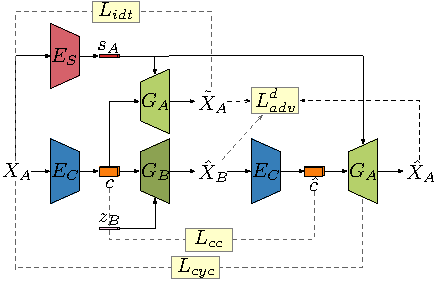
\includegraphics[width=1\textwidth]{figures/G.pdf}
    \caption{水下图像多模态转译模型MUGAN转译器网络结构。}
    \label{fig:mugan_g}
\end{figure*}

我们设置图像集$A$和$B$分别为空中域和多模态水下域。输入不配对的图像$x_A \in A$和$x_B \in B$,我们的目标是训练一个网络结构使得网络结果能够学会生成目标域$B$的多模态结果,且多模态结果对应于输入图像$A$的内容。多样的域风格向量可以来自目标域分布的随机采样也可以来自给定图像编码。

图~\ref{fig:mugan_g}和图~\ref{fig:mugan_d}所示为水下图像多模态转译模型MUGAN网络结构。MUGAN网络结构基于分解表达学习,图~\ref{fig:mugan_g}是转译模型结构,图~\ref{fig:mugan_d}是判别结构。转译模型包括编码器和生成器,生成器结构有两个分支,上分支整体来看是一个编码器-解码器结构,下分支整体是一个类似CycleGAN的循环网络,目的是训练模型实现跨域转译。

\begin{figure*}[ht]
    \centering
    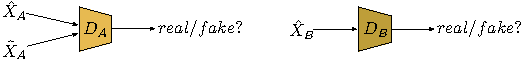
\includegraphics[width=1\textwidth]{figures/D.pdf}
    \caption{水下图像多模态转译模型MUGAN判别器网络结构。}
    \label{fig:mugan_d}
\end{figure*}

\textbf{编码器。}编码器包括两个,一个是内容编码器,一个是风格编码器。给一张来自空中域的图像$x_A$或者水下多模态域的图像$x_B$,风格编码器$E_S$提取给定图像的风格编码$s_A$或者$s_B$,其中$s_A = E_S(x_A)$,$s_B = E_S(x_B)$。内容编码器$E_C$将图像编码至内容空间$C$中。如图~\ref{fig:mugan_g}所示,内容编码器$E_C$将$x_A$编码成内容向量$c$,来自$\hat{x_B}$的向量$\hat{c}$理论上跟来自$x_A$的向量$c$是一致的,只是域风格信息不一致。$E_S$是一个MLP映射网络,$E_C$是一个包括三个卷集模块和四个残差模块的网络。

\textbf{生成器结构。}我们的生成器$G_A(\cdot)$和$G_B(\cdot)$将输入的内容和风格转译到目标域,目标域具有的特定风格特征信息可以来自目标域特定分布的采样$z_A$和$z_B$或者风格编码器提取的风格编码$E_S(\cdot)$。我们生成器包挎四个残差模块和两个上采样模块。我们对上采样模块和残差模块分别使用实例归一化(IN)和自适应实例归一化(AdaIN)~\cite{huang2017arbitrary}。风格信息通过全部AdaIN层注入,通过学习仿射变换进行缩放和移动向量。

\textbf{判别器结构。}判别器$D_A$和$D_B$都是PatchGAN~\cite{isola2017image}网络。判别器$D_A$用来判断输入图像$x$是来自$A$域的真实样本还是$A$域生成器$G_A$的生成结果$G_A(c,s_A)$,相应地判别器$D_B$是用来判断输入图像$x$是来自$B$域的真实样本还是$B$域生成器$G_B$的生成结果$G_B(\tilde{c},z_B)$。

\subsection{目标函数和算法}
$A$域和$B$域分别为空中域和水下多模态域,给定图像$x_A \in A$和输入目标域风格随机采样编码$z_B$,我们训练从$A \rightarrow B$的方向上的转译,其中用到的目标函数如下所示。

\textbf{域对抗损失。} 训练过程中,翻译器网络输入纯净完整的内容信息和目标域风格信息,通过域对抗损失限制翻译器学习生成目标域结果

\begin{equation}
\label{equ:adv_a_}
\mathcal{L}_{adv}^{\tilde{x}_A} = \mathbb{E}[\log D_A(x_A)] + \mathbb{E}[\log(1-D_A(G_A(c,s_A)))]
\end{equation}

\begin{equation}
\label{equ:adv_a}
\mathcal{L}_{adv}^{\hat{x}_A} = \mathbb{E}[\log D_A(x_A)] + \mathbb{E}[\log(1-D_A(G_A(\hat{c},s_A)))]
\end{equation}

\begin{equation}
\label{equ:adv_b}
\mathcal{L}_{adv}^{\hat{x}_B} = \mathbb{E}[\log D_B(x_B)] + \mathbb{E}[\log(1-D_B(G_B(c,z_B)))]
\end{equation}

生成器$G_A$学习使用来自$A$域的风格样式$s_A$生成$A$域具有足够真实性的图像$G_A(c,s_A)$和$G_A(\hat{c},s_A)$,企图可以混淆真实图像和生成结果,让$A$域判别器$D_A$无法区分他们。类似地,生成器$G_B$学习使用目标域分布采样编码$z_B$合成$B$域具有真实性的图像结果$G_B(c,z_B)$,目标也是让$B$域判别器$D_B$无法区分输入是真实图像还是生成假结果。

\textbf{循环一致性损失。}为了保证$A \rightarrow B$和$B \rightarrow A$两个方向上映射是循环一致的,我们使用CycleGAN~\cite{zhu2017unpaired}中提出的循环一致性损失来进行限制。

\begin{equation}
\label{equ:cycle}
\mathcal{L}_{cyc} = \mathbb{E}[\| G_A(\hat{c}, s_A) - x_A \|_1]
\end{equation}

其中$G_A(\hat{c}, s_A)$是$x_A$的重建结果。

\textbf{同一性损失。}我们在真实样本和生成结果$G_A(c,s_A)$之间采用同一性映射

\begin{equation}
\label{equ:idt}
\mathcal{L}_{idt} = \mathbb{E}[\| G_A(c, s_A) - x_A \|_1]
\end{equation}

当编码器成功地将输入图像分解成内容和风格两部分信息,理论上输入的真实数据应该跟合成的$G_A(c,s_A)$之间的距离非常接近。该损失保证生成器$G_A(\cdot)$生成$A$域的风格,不会自主地修改图像的色调,使得整体的风格产生变化。

\textbf{内容一致性损失。}为了保证从源域到目标域的跨域转译过程中内容保持完整,目标函数加入内容一致性损失,即真实样本和生成结果经过内容编码器分解得到的内容向量所包含的信息应该是一致的。

\begin{equation}
\label{equ:cc}
\begin{aligned}
\mathcal{L}_{cc} & = \mathbb{E}[\| E_C(G_A(c, s_A)) - E_C(x_A) \|_1] \\
       & = \mathbb{E}[\| \hat{c} - c \|_1]
\end{aligned}
\end{equation}

\textbf{KL损失。}KL损失致力于将分解后的内容和风格表达对齐高斯先验分布。

\textbf{总目标函数。}我们总的目标函数可以概括如下:

\begin{equation}
\label{equ:full}
\begin{aligned}
\min_{E,G}\max_{D} & \mathcal{L}_{adv}^{\tilde{x}_A}+\mathcal{L}_{adv}^{\hat{x}_A}+\mathcal{L}_{adv}^{\hat{x}_B} \\
+&\lambda_{cyc}\mathcal{L}_{cyc}+\lambda_{idt}\mathcal{L}_{idt}+\lambda_{cc}\mathcal{L}_{cc}+\lambda_{kl}\mathcal{L}_{kl}
\end{aligned}
\end{equation}

其中$\lambda_{cyc}$,$\lambda_{idt}$,$\lambda_{cc}$和$\lambda_{kl}$是对应每单项损失的超参数。后续除了分布采样向量,我们还用引导图像经过经过风格编码器后得到风格编码来测试我们模型的有效性。我们默认设置这些参数分别为$10$,$5$,$1$,$0.01$。

\section{水下图像多样式域转译设计}
在这一节,将对该问题进行分析,提出模型设计思路,设置目标函数,为下一章节中的实验提供理论依据和实验意义。

\subsection{问题及分析}
我们将给定图像转译到水下环境的多样式域的图像转译称为水下图像多样式域转译。基于生成对抗网络,我们想通过一个网络结构,在无监督的条件下,实现水下图像多样式域的图像转译。受UIE-DAL方法启发,通过对多个水下条件进行编码,从而对多个样式域进行控制,实现到多个样式域的转译。

对图像转译中的经典方法综述。CycleGAN是经典跨域转译方法,通过循环一致性损失成功实现两个域之间的双向转译,想要实现多域之间的转译,只能一一之间进行训练,若有$n$个域之间转译,需要训练$n(n-1)/2$次。StarGAN解决了多域转译的问题,只使用一个生成器来实现多个域之间的生成。在StarGAN中,并不使用传统的固定转译,而是将域信息和图片一起输入进行训练,并在域标签中加入编码向量,便于不同的训练集进行联合训练。通过加入每个域设置的标签,对应的把生成图片变到指定的域。StarGAN v2在StarGAN实现多域转译的基础上,同时解决生成图像的多样性和在多个域上的可扩展性的问题。以StarGAN为基础,用特定域的样式代码替换原来的域标签,这些代码可以表示特定域的各种形式。StarGAN v2引入两个模块,一个映射网络将随机高斯噪声转换为样式代码和一个样式编码器从给定的参考图像中提取样式代码。DRIT++在DRIT两个域多模态转译的基础上拓展至多个域之间的图像转译。给每个域进行one-hot编码,加入域分类损失,以区分不同域。在作者给出的代码中单独为多域转译任务建立一个项目称MDMM,后续会用MDMM作为DRIT++工作中多域转译方法。

%这些方法测试结果中存在的问题。
%我们设置的方法好处
在用多域转译方法解决我们转译到水下多个样式条件下图像问题时,我们设计了一个多域转译模型。使得在转移过程中目标内容保持不变,多个样式域仅仅改变图像中的水下环境条件。在不需要配对数据的情况下,给定要转译的多个域图像,通过对各个域进行编码作为域控制条件,实现到多个样式域的转译任务,对数据配对没有要求,有很强的泛化能力。

\subsection{模型结构}

\begin{figure*}[ht]
    \centering
    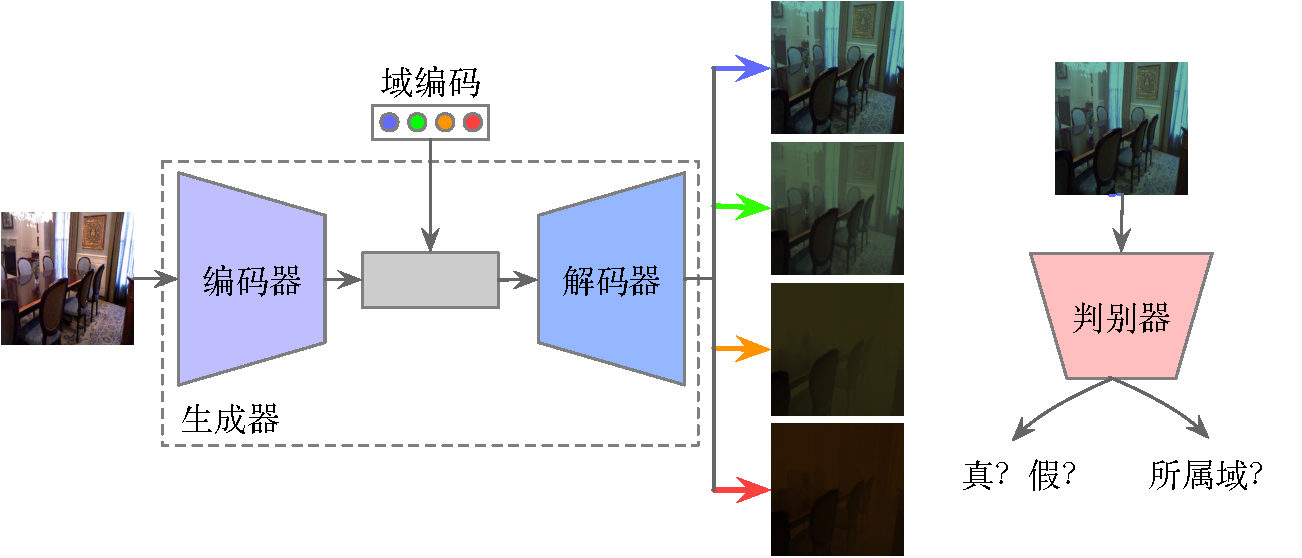
\includegraphics[width=1\textwidth]{figures/Domain_network.pdf}
    \caption{水下图像多样式域转译网络结构。}
    \label{fig:domain_net}
\end{figure*}

我们设置输入数据Input,其他样式的数据分别作为$A$,$B$、$C$、$D$等依次顺序排列域。我们的目标是通过网络结构使得输入能够学会转译到各个域中,其中转译结果中的内容跟输入保持一致,不同的域之间只有样式发生变化,样式可以是浑浊度、颜色等视觉效果变量。

图~\ref{fig:domain_net}所示为水下图像多样式域转译模型的网络结构。左边是生成器模型结构,右边是判别器模型结构。生成器结构是一个基于卷积神经网络的编码器-解码器结构,编码器进行下采样将输入图像特征提取,采样至潜在编码空间,解码器进行上采样,将潜在编码向编码的目标域进行转译,输入图像通过输入的域编码控制来合成对应域样式的结果。判别器结构负责多任务判断,除了判别输入样本的真假之外还要判断该样本属于哪一个样本域。

\subsection{目标函数和算法}
在多样式域转译模型中,我们训练生成器结构将输入图像$x$转译至目标域$c$的相应输出$G(x,c)$。判别器结构一方面用来判断输入结果的真假概率$D(x)$,另一方面还判断输入样本的所属域$D_cls(x)$。

\textbf{对抗损失。}为了使生成样本趋近于真实样本,让判别网络无法区分,我们采用对抗损失 

\begin{equation}
\label{equ:adv_exp2}
\mathcal{L}_{adv} = \mathbb{E}_x[\log D(x)] + \mathbb{E}_{x,c}[\log(1-D(G(x,c)))]
\end{equation}

其中生成器使用输入图像$x$和目标域编码$c$来合成图像$G(x,c)$,判别器尝试去判断输入是真实样本还是合成样本。生成器尝试去最小化这个函数,判别器尝试去最大化函数。

\textbf{域分类损失。}我们希望生成器合成的图像结果$G(x,c)$能够正确分类到目标域$c$中。为了达成这个目标,我们的判别器结构也能进行域分类,真实样本的域分类损失来优化判别器,合成样本的域分类损失来优化生成器。

真实样本的域分类损失为

\begin{equation}
\label{equ:cls_real_exp2}
\mathcal{L}_{cls}^{r} = \mathbb{E}_{x,c'}[-\log D_{cls}(c'|x)]
\end{equation}

$D_{cls}(c'|x)$这项表示由$D$计算的域标签上的概率分布。通过最小化这项损失,$D$学会去区分真实样本和它所属域$c'$,输入图像$x$和它对应的域标签$c'$在数据集训练时设置。另一方面,生成样本的域分类损失为

\begin{equation}
\label{equ:cls_fake_exp2}
\mathcal{L}_{cls}^{f} = \mathbb{E}_{x,c}[-\log D_{cls}(c|G(x,c))]
\end{equation}

生成器$G$尝试去最小化这个损失,使得合成图像能够被分类到目标域$c$。

\textbf{重建损失。}通过最小化对抗损失和域分类损失,生成器$G$训练生成真实和正确域的结果。需要通过一个限制来保证转译过程中内容不变,只有域样式发生变化,我们借鉴循环一致性损失来作为这个限制

\begin{equation}
\label{equ:rec_exp2}
\mathcal{L}_{rec} = \mathbb{E}_{x,c,x'}[\| x-G(G(x,c),c') \|_1]
\end{equation}

生成器$G$将合成结果$G(x,c)$和$x$的原始域作为输入,试图去重建原始图像$x$。我们采用$L_1$归一项作为重建损失。

\textbf{总目标函数。}生成器$G$和判别器$D$的目标函数分别如下

\begin{equation}
\label{equ:D_exp2}
\mathcal{L}_{D} = -\mathcal{L}_{adv} + \lambda_{cls}\mathcal{L}_{cls}^{r}
\end{equation}

\begin{equation}
\label{equ:G_exp2}
\mathcal{L}_{G} = \mathcal{L}_{adv}+\lambda_{cls}\mathcal{L}_{cls}^{f}+\lambda_{rec}\mathcal{L}_{rec}
\end{equation}

其中$\lambda_{cls}$和$\lambda_{rec}$是对应每单项损失的超参数,其权重对应相比于对抗损失的重要性来进行设置。在所有实验中,我们默认设置$\lambda_{cls}=1$,$\lambda_{rec}=10$。


\section{实验环境}
整个网络使用Pytorch框架,计算机环境CPU型号为Intel$^\circledR$ Core$^{\text{TM}}$ i5-8500 CPU,操作系统为Ubuntu 16.04 LTS版本,显卡型号为Nvidia GeForce GTX 1070,内存128GB,显存为8GB。

本工作中使用的基准方法模型使用官方Github中给出的Pytorch版本代码进行实验。根据代码中需要的依赖包,使用Anaconda创建和控制相应的虚拟环境实验。为了彰显公平,在选取基准方法时,全部选择给出完整版本代码的方法进行对比。

\section{本章小结}
经典的水下多样式图像合成方法,一种是基于光学物理模型将深度图或者传输图等水下信息带入合成图像中,合成特定水下信息的结果,合成结果与带入水下条件信息一一对应;另一种是基于无监督图像转译模型CycleGAN,空中域和水下特定样式域作为CycleGAN跨域转译的两个域,可以实现从空中图像到特定水下样式域的转译,合成结果在水下特定样式域分布中,输入和输出结果一一对应。这些方法都无法一次获得多样式结果。因此,在水下环境中,给定不配对样本,将输入一次转译成多种水下样式结果就是一个很关键的问题,是解决许多水下视觉任务的重要问题。

如在上一章最后一小节,我们想通过两种思路来解决这个问题。在这一章中,我们将两种思路进行分析,设计出可行的网络结构,设置相应的目标函数,为后续实验提供理论依据和实验意义。

本章第一节介绍了水下图像跨域多模态转译设计,将水下图像多样式合成任务用跨域多模态转译模型来实现,水下的多种样式看作水下域的多个模态。在经典的跨域多模态转译方法中,这些方法在解决该问题时会有失败案例出现,针对这些问题我们设计了一个基于分解表达学习的模型,详细介绍了模型结构和各部分组成的实现,引入内容一致性损失来限制转译过程中内容保存不完整的问题,多种损失共同限制解决水下图像跨域多模态转译问题。

本章第一节介绍了水下图像多样式域转译设计,将水下图像多样式合成任务用多域转译模型来实现,空中域和多个水下样式都各自看成一个域。多个经典多域转译模型在解决该问题时,会有各自限制。我们设计了一个水下多样式域转译模型,将转译模型的主要网络结构进行了介绍,并将各种目标函数进行设置。

本章第三节介绍了我们的实验环境,为了保证了后续实验的客观公正,实验中代码使用相同框架和相同的实验环境。
